%!TEX program = xelatex

\documentclass[letterpaper,11pt]{extarticle}
% Euler math font
\usepackage{eulervm}
\usepackage[T1]{fontenc}

% General
\usepackage[no-math]{fontspec} % Specify fonts
\usepackage[english]{babel}    % Naming of figures and such
\usepackage[
    style=ieee,
    sortlocale=en_GB
    ]{biblatex}                % Bibliography styling
\usepackage{import}            % Importing subdocuments
\usepackage{standalone}        % Compilable subdocuments
\usepackage{hyperref}          % Clickable references
\usepackage{csquotes}          % Required for biblatex

% Page layout
\usepackage[
    a4paper,
    bottom=1.2in,
    top=1.2in,
    left=0.8in,
    right=0.8in,
    headheight=14pt
    ]{geometry}               % Margins
\usepackage{fancyhdr}         % Header
\usepackage{lastpage}         % Page numbers in footer
\usepackage{setspace}         % Line spacing
\usepackage{ragged2e}         % Better line endings
\usepackage[parfill]{parskip} % New line instead of indentation
\usepackage{titlesec}         % Size of sections

% Utility
\usepackage[table]{xcolor}                                       % Colors
\usepackage[separate-uncertainty=true, per-mode=symbol]{siunitx} % Display units
\usepackage{enumitem}                                            % Better enumeration
\usepackage{ifthen}                                              % If-statements
\usepackage{lipsum}                                              % Lorem ipsum
\usepackage{algpseudocode}
\usepackage{algorithm}

% Figures
\usepackage{pgfplots}                   % Plots
\pgfplotsset{compat=newest}             % Pgfplots compatibility
\usepackage{tikz}                       % Tikz figures
\usepackage{float}                      % Floating of figures
\usepackage{ltablex}                    % Merge of tabularx and longtable (use tabularx if stuff breaks)
\usepackage{multirow}                   % Cells spanning multiple rows
\usepackage{graphicx}                   % Graphics
\usepackage{caption}                    % Subfigures and captions
\captionsetup{justification=centering}
\usepackage{subcaption}                 % Subfigures and captions
\usepackage{booktabs}                   % Toprule etc
\usepackage{wrapfig}                    % Wrapping around figures if necessary

% Math
\usepackage{amsmath} % Math commands
\usepackage{amsthm}         % Math environments
\usepackage{amssymb}        % Math symbols

% Cleveref
\usepackage[noabbrev, capitalize]{cleveref} % Automatic referencing

% Custom math
% Vectors
\renewcommand{\vec}[1]{\boldsymbol{#1}} % Vector
\newcommand{\vecu}[1]{\hat{\vec{#1}}}   % Unit vector
\newcommand{\mat}[1]{\vec{#1}}          % Matrix

% Set notations
\newcommand{\Z}{\mathbb{Z}}   % Integers
\newcommand{\R}{\mathbb{R}}   % Real numbers
\renewcommand{\C}{\mathbb{C}} % Complex numbers
\newcommand{\N}{\mathbb{N}}   % Natural numbers

% Symbols
\newcommand{\es}{\varnothing}   % Empty set
\newcommand{\e}{\varepsilon}    % Epsilon
\newcommand{\sub}{\subseteq}    % Subset
\newcommand{\imp}{\Rightarrow}  % Implication
\renewcommand{\d}{\partial}     % Partial
\renewcommand{\th}{\theta}      % Theta

% Operators
\renewcommand{\Re}{\operatorname{Re}}
\renewcommand{\Im}{\operatorname{Im}}
\newcommand{\Cov}{\operatorname{Cov}}
\newcommand{\Var}{\operatorname{Var}}
\newcommand{\argmax}[1]{\underset{#1}{\operatorname{argmax}}~}
\newcommand{\argmin}[1]{\underset{#1}{\operatorname{argmin}}~}
\newcommand{\tr}{\operatorname{tr}}
\newcommand{\col}{\operatorname{col}}
\newcommand{\proj}{\operatorname{proj}}
\renewcommand{\perp}{\operatorname{perp}} % \bot for perp symbol
\newcommand{\sign}{\operatorname{sign}}
\newcommand{\rank}{\operatorname{rank}}

% Small superscript in math
\newcommand{\sus}[1]{^{\text{\tiny $#1$}}}
\newcommand{\supsmall}[1]{\sus{#1}}        % Explicit command

% Subscripts without spacing
\renewcommand{\ss}[1]{_\mathit{#1}}

% Straight 'd' in integral
\newcommand{\id}[1]{\, \mathrm{d} #1}

% Amsmath environements
\newtheorem{theorem}{Theorem}
\newtheorem{lemma}{Lemma}
\newtheorem{definition}{Definition}

% Fix interference of parfill option of parskip package with amsmath environments
\begingroup
    \makeatletter
    \@for\theoremstyle:=definition,remark,plain\do{%
        \expandafter\g@addto@macro\csname th@\theoremstyle\endcsname{%
            \setlength\thm@preskip\parskip
            \setlength\thm@postskip{0pt}
            \addtolength\thm@preskip\parskip
            }%
        }
\endgroup


% Hyperlink
\hypersetup{
    colorlinks,
    citecolor = black,
    filecolor = black,
    linkcolor = black,
    urlcolor  = black
}

% Left-justified text in tabularx environment
\newcolumntype{L}{>{\RaggedRight\arraybackslash}X}

% Fonts
\setsansfont{Avenir Next LT Pro}
\setromanfont{Adobe Caslon Pro}
\setmonofont[Scale=0.85]{Source Code Pro}
\newcommand{\code}[1]{\texttt{#1}} % Code

% Style enumerate
\setlist[enumerate]{label=(\arabic*)}
\setlist[itemize]{label=\textbullet}

% Shortcuts to colors
\newcommand{\red}[1]{{\color{red} #1}}
\newcommand{\blue}[1]{{\color{blue} #1}}
\newcommand{\green}[1]{{\color{green} #1}}

% Line spacing
\onehalfspacing

% Page layout
\pagestyle{fancy}
\lhead{\DocTitle\ifthenelse{\equal{\DocCourse}{}}{}{, \DocCourse}}
\chead{}
\rhead{\DocAuthor}
\lfoot{}
\cfoot{}
\rfoot{Page~\thepage~of~\pageref{LastPage}}
\renewcommand{\headrulewidth}{0pt}
\renewcommand{\footrulewidth}{0pt}

\newcommand{\DocCourse}{}
\newcommand{\DocTitle}{}
\newcommand{\DocAuthor}{}

% Title and sections
\titleformat*{\section}{\Large\bfseries}
\titlespacing*{\section}{0pt}{\baselineskip}{0.5\baselineskip}
\titleformat*{\subsection}{\large\bfseries}
\titlespacing*{\subsection}{0pt}{\baselineskip}{0.5\baselineskip}
\renewcommand{\title}{\vspace*{-1.4em}{\LARGE\bfseries\DocTitle}\vspace*{0.5\baselineskip}}

% Sections in margins
\newcommand{\sectionsInMargins}{
    \titleformat{\section}[leftmargin]
        {\Large\bfseries\filleft}
        {\thesection) }{0pt}{}
        \titlespacing{\section}
        {4pc}{1.5ex plus .1ex minus .2ex}{1pc}
}
\newcommand{\subsectionsInMargins}{
    \titleformat{\subsection}[leftmargin]
        {\large\bfseries\filleft}
        {\thesubsection) }{0pt}{}
        \titlespacing{\subsection}
        {4pc}{1.5ex plus .1ex minus .2ex}{1pc}
}

% Run in on sections
\newcommand{\runInSection}{
    \titleformat{\section}[runin]
        {\normalfont\Large\bfseries}{\thesection}{1em}{}
}

\newcommand{\runInSubsection}{
    \titleformat{\subsection}[runin]
        {\normalfont\Large\bfseries}{\thesubsection}{1em}{}
}

% Reduced space below figures
% \setlength{\belowcaptionskip}{-1em}

% Easy section creation
\newcommand{\newSection}[1]{\section{} \label{sec:#1}}

% Listings
\usepackage{listings}
\newcommand\listingStyle{\lstset{
    otherkeywords    = {self},
    basicstyle       = \fontsize{9}{8}\selectfont\ttfamily,
    showstringspaces = false,
    breaklines       = true,
    postbreak        = \raisebox{0ex}[0ex][0ex]{\ensuremath{\color{red}\hookrightarrow\space}},
    tabsize          = 2,
    escapeinside     = {(*}{*)},
    mathescape
}}

\lstnewenvironment{listing}[1][]
  {\vspace{0.25em}\listingStyle\lstset{#1}}
  {\vspace{-0.75em}}


% Table footnote
\newcommand{\tableFootnote}[1]{
    \\[0.5em]
    {\centering \footnotesize #1}
    \vspace{-0.5em}
}

% Scientific e notation
\newcommand{\sce}{\text{\sc{e}}}

% Framed listing
\newcommand{\framedListings}{
    \lstset{
         frame     = single,
         framerule = 0.075em,
         rulecolor = \color{black}
    }
}

% Floating listings
\DeclareCaptionFormat{cont}{#1~(cont.)#2#3 }

\newcounter{tmp}

\newcommand\savecount{\setcounter{tmp}{\value{lstlisting}}}
\newcommand\contcap{%
\setcounter{lstlisting}{\value{tmp}}
\addtocounter{lstlisting}{-1}
\captionsetup[lstlisting]{format=cont}}

% Expandable input
\makeatletter
\newcommand*\expandableInput[1]{\@@input#1 }
\makeatother

\addbibresource{bibliography.bib}

\renewcommand{\DocTitle}{Coursework 2}
\renewcommand{\DocCourse}{MLSALT6}
\renewcommand{\DocAuthor}{James Requeima (jrr41), Wessel Bruinsma (wpb23)}

\usepackage{setspace}

\newcommand{\outputPath}{output/}

\begin{document}
\title
\singlespacing

\begingroup

In this document we briefly describe the design of the Adaptive Run-length Huffman Compressor (ARHC).

\section{Motivation}
% For the task of compressing $N=10,000$ bits, each having probability $p = 0.01$ of being a 1, the extra bit overhead of the Huffman algorithm prohibits naive application of it. Since the $0$ symbol is highly probable, its observations conveys virtually no information. On If we are observing the file bit-by-bit, the number of bits that pass before a one is observed does contain a lot of information. As an approach, we treat each of these zero-counts, or run-lengths, as a symbol for the Huffman algorithm. To make sure that our encoding and decoding algorithm is well defined, we pick a maximum run-length $n$ that defines the largest number of zeros denoted as a symbol. More precisely, let
For the task of compressing $N=10,000$ bits, each having probability $p = 0.01$ of being a 1, the extra bit overhead of the Huffman algorithm prohibits naive application of it; since the $0$ symbol is highly probable and thus its observation conveys virtually no information, encoding it by a bit is wasteful.

Imagine that we observe the input file bit by bit. Then the numbers of bits that pass before ones are observed fully describe the file, and in addition all have high information content. This motivates the approach to define each of these zero-counts, also called run-lengths, as the symbols of our alphabet. However, to make sure that our approach is well defined, we pick a maximum run-length $n$ that defines the largest number of zeros denoted as a symbol. More precisely, let
\begin{align*}
    \mathcal{A}_X &= \big(1, 01, 001, \ldots, \underbrace{0\cdots0}_{n-1}\!1, \underbrace{0\cdots0}_{n} \big), \\
    \mathcal{P}_X &= \big( p, (1-p)p, \ldots, (1-p)^{n-1}p, (1-p)^n \big)
\end{align*}
be the ensemble that will be encoded by a Huffman code $C_X$.

It remains to determine an appropriate maximum run-length. Let $L$ denote the expected codelength and let $H$ denote the entropy of the distribution over the symbols in our symbol set. Then the expected number of wasted bits per symbol is  $L - H$. The red line in \Cref{fig:ratio} shows the ratio $L/H$ where $L$ is determined by explicitly computing the Huffman code for the associated $n$, and the dashed green line shows an approximation.\footnote{We can determine the optimal run-length observed in \cref{fig:ratio} by approximating the behaviour of the Huffman algorithm. First we exploit the structure of the symbols in $\mathcal{A}_X$ and decompose the entropy via
\begin{align*}
    H(X) = \underbrace{H_2(p) + p(H_2(p) + p(H_2(p) + \ldots))}_{n~\text{terms}}
    = H_2(p) \sum_{i=0}^{n-1} p = \frac{H_2(p)}{p}(1-(1-p)^n).
\end{align*}
Motivated by the fact that $1-p$ is small, we assume that the result of running the Huffman algorithm on the first $n$ symbols in $\mathcal{A}_X$ is similar to the result if they have equal probability. Now Exercise 5.28 in \cite{mackayinformation} yields that the first $\lfloor (n-1) f^- \rfloor$ symbols in $\mathcal{A}_X$ will have length $\lfloor \log_2 (n - 1) \rfloor + 1$ and the other  $n - 1 -\lceil (n-1) f^- \rceil$ symbols in $\mathcal{A}_X$ will have length $\lceil \log_2 (n - 1) \rceil + 1$ where $f^- = 2^{\lceil \log_2 (n - 1) \rceil}/(n-1) - 1$. We can then approximate the expected length by
\begin{align*}
    L \approx \sum_{i=1}^{\lfloor (n-1) f^- \rfloor} (1-p)^{i-1}p\cdot (\lfloor \log_2 (n - 1) \rfloor + 1) +
    \sum_{i=\lceil (n-1) f^- \rceil}^{n} (1-p)^{i-1}p\cdot (\lceil \log_2 (n - 1) \rceil + 1) + (1-p)^n.
\end{align*}
The approximation of $L/H$ using the above expression for $H$ and above approximation for $L$ is shown by the dashed green line in \cref{fig:ratio}. We see that the approximation holds perfectly for $n \le 100$ where inspection of the computed Huffman codes shows that the assumption indeed holds.} We see that this ratio attains extrema at multiples of $69$ and that $L$ closely approximates $H$ at these points. Now the expected codeword length of the Huffman code is equal to the entropy when the distribution over the symbols in our symbol set is dyadic. Therefore, since all-zero symbol has probability $0.99^n$, in order to have $L/H$ close to one, we must have that $0.99^n \approx 2^{-k}$ for any natural $k$, which implies that $n \approx k\times 69$. We choose to use $n=69$.

\begin{figure}[ht]
    \centering
    \includegraphics[width=\linewidth]{\outputPath optimal_n}
    \caption{Ratio $L/H$ for different run-lengths $n$}
    \label{fig:ratio}
\end{figure}


\section{Description}
\Cref{alg:pseudo} provides a high-level overview of ARHC. Descriptions of the components of the program can be found in the source code or in the documentation in \code{documentation.epub}.

The implementation of the Huffman algorithm is facilitated through \code{Leaf} and \code{Node} objects that define a binary tree. The algorithm is initialised by encapsulating each symbol and its probability in a \code{Leaf} object, and the merge operation is performed by combining two \code{Leaf} objects into a \code{Node} object. A code word can be mapped to its symbol by providing it as an argument to the \code{decode} operation of the root \code{Node} of the tree. Additionally, the encoding of all code words can be obtained by calling the \code{getEncoding} operation of the root \code{Node} of the tree.

If $p$ is unknown, then the user can provide parameters $\alpha_0$, $\alpha_1$ for a prior $\operatorname{Beta}(\alpha_0, \alpha_1)$ over $p$. In lines 17 to 19 of \cref{alg:pseudo}, the posterior over $p$ is updated according to the observation $S$.

The operation of line 6 of \cref{alg:pseudo} dynamically adjusts the run-length so that
\begin{enumerate}
    \item the run-length is near optimal for the current estimate of $p$ and
    \item the symbols in $\mathcal{A}_X$ are able to entirely encode and decode the input stream\footnote{When $n>N$, then $\mathcal{A}_X$ might not be able to encode the remaining bits in the input stream, and some symbols in $\mathcal{A}_X$ will never be used.} without the use of an end-of-transmission symbol or the length of the transmitted message.
\end{enumerate}

Note that ARHC is able to perform partial compression and partial decompression; the compressor writes a symbol directly after the associated input bits are read and similarly the decompressor writes the input bits directly after the associated symbol is read. We will experiment with this behaviour by feeding the input bit by bit in \cref{sec:analysis}.

\begin{algorithm}[ht]
    \begin{algorithmic}[1]
        \Function{arhc}{$I$, $O$, $N$, $p$ or ($\alpha_0$ and $\alpha_1$)} \Comment{$I$ represents the input stream and $O$ represents the output stream}
            \If{adaptation}
                \State $p \gets \alpha_1 / (\alpha_0 + \alpha_1)$
            \EndIf
            \While{$N > 0$}
                \State $n \gets \max\{1,\min\{\operatorname{round}(-1/\log_2 (1 - p)) , N\}\}$
                \State Obtain the code $C_X$ by running Huffman algorithm on the ensemble \begin{align*}
                    \mathcal{A}_X &= \big(1, 01, 001, \ldots, \underbrace{0\cdots0}_{n-1}\!1, \underbrace{0\cdots0}_{n} \big), \\
                    \mathcal{P}_X &= \big( p, (1-p)p, \ldots, (1-p)^{n-1}p, (1-p)^n \big)
                \end{align*}
                \If{compression}
                    \State $S \gets$ Read from $I$ the first symbol that corresponds with a symbol in $\mathcal{A}_X$
                    \State Write to $O$ the code word of $S$ according to $C_X$
                \ElsIf{decompression}
                    \State $S \gets$ Read from $I$ the first symbol that corresponds with a code word in $C_X$
                    \State Write to $O$ the symbol of $S$ in $\mathcal{A}_X$ according to $C_X$
                \EndIf
                \State $N \gets N - \operatorname{length}(S)$
                \If{adaptation}
                    \State $\alpha_0 \gets \alpha_0 + \operatorname{count}_0(S)$
                    \State $\alpha_1 \gets \alpha_1 + \operatorname{count}_1(S)$
                    \State $p \gets \alpha_1 / (\alpha_0 + \alpha_1)$
                \EndIf
            \EndWhile
        \EndFunction
    \end{algorithmic}
    \caption{Adaptive Run-length Huffman Compressor}
    \label{alg:pseudo}
\end{algorithm}

\section{Analysis}
\label{sec:analysis}
The source coding theorem tells us that we cannot compress the $N$-bits input further than $NH_2(p)\approx807.9$ bits. We can approximate the length of the compressed input by $\hat{N}=NL/L_i$ where $L_i$ represents the expected number of inputs bits a symbol in $\mathcal{A}_X$ represents. We calculate $L_i$ via
\begin{align*}
    L_i = \sum_{i=1}^{n-1}(1-p)^{i-1}p\cdot i +(1-p)^n\cdot n
\end{align*}
which yields for $n=69$ that $\hat{N}=810.5$ bits; by averaging over 500 runs we indeed found that $\hat{N}\approx 812.3$. \Cref{tab:compression_performance} shows an overview of the compression performance of ARHC.

\begin{table}[ht]
    \centering
    \begin{tabular}{l|ll}
        \toprule
        & Compressed input & Compression ratio \\ \midrule
        Optimal & $807.9$ bits & $0.9192$ \\
        ARHC & $810.5$ bits & $0.9190$ \\ \bottomrule
    \end{tabular}
    \caption{Compression performance of ARHC}
    \label{tab:compression_performance}
\end{table}

\Cref{fig:different_N} shows the compression performance of the static and adaptive compression scheme for different inputs lengths $N$. We see that the static compression scheme converges to the optimal compression rate more quickly than the adaptive compression scheme, but that the adaptive compression scheme has initially lower variance. This reflects the classical convergence speed versus variance tradeoff.

\Cref{tab:bits_highlight} shows the output of the compressor and decompressor when the input is fed bit by bit.\footnote{Feeding the compressor and decompressor bit by bit turned out to be quite a challenge; it required us to flag the input and output streams as non-blocking and take into account the processing time of the compressor.} It shows the case where the parameter $p$ of the static compression scheme matches the probability of the bent coint and the case where it does not. We see that in the former case the static compression scheme converges more quickly to the optimal compression ratio than the adaptive compression scheme, though with higher variance, but that in the latter case the adaptive compression scheme is able to adapt to the mismatched probability and eventually outperform the static compression scheme.

\Cref{fig:comparison_priors} shows the effect of different settings of $\alpha_0$ and $\alpha_1$ on the performance of the adaptive compression scheme when the input is fed bit by bit. We see that for small $\alpha_0$ and $\alpha_1$ the compressor is able to more quickly adapt, but also has higher variance. This again reflects the classical convergence speed versus variance tradeoff.

Finally, \cref{tab:bits_highlight} shows the output of the compressor and decompressor when the input is fed bit by bit. This allows us to concretely inspect the dynamics of the adaptive compression scheme. We see that as the adaptive compressor sees more bits, it learns to efficiently encode the all-zero symbol.

\begin{figure}[ht]
    \centering
    \includegraphics[width=\linewidth]{\outputPath Ns.pdf}
    \caption{Compression performance of the static and adaptive compression scheme for different input lengths $N$}
    \label{fig:different_N}
\end{figure}


\begin{table}[ht]
    \centering
    \vspace{-0.55cm}
    \setstretch{0.55}
    \centerline{\hspace{.5cm}\begin{subfigure}{.6\linewidth}
        \begin{tabular}{lp{3cm}p{4cm}}
            \toprule
            Input bit & Compressor output & Decompressor output \\ \midrule
            \expandableInput{\outputPath tab_static.tex}
            \bottomrule
        \end{tabular}
        \hspace{1cm}\caption{Static compression scheme}
    \end{subfigure}
    \begin{subfigure}{.6\linewidth}
        \begin{tabular}{lp{3cm}p{4cm}}
            \toprule
            Input bit & Compressor output & Decompressor output \\ \midrule
            \expandableInput{\outputPath tab_adaptive.tex}
            \bottomrule
        \end{tabular}
        \caption{Adaptive compression scheme}
    \end{subfigure}}
    \caption{Output of the compressor and decompressor when the input is fed bit by bit. The input consists of the first 80 bits of the bent-coin benchmark file \code{filep.01.10000NR}. The parameters of the prior are $\alpha_0=0.2$ and $\alpha_1=0.2$. The static compression scheme compresses down to 22 bits, the adaptive compression scheme compresses down to 23 bits and the SCT tells us that we cannot compress further than $80 H_2(0.01) \approx 6.5$ bits.}
    \label{tab:bits_highlight}
\end{table}


\begin{figure}[ht]
    \centering
    \begin{subfigure}{.49\linewidth}
        \includegraphics[width=\linewidth]{\outputPath comparison1}
        \caption{Compressor matches reality, the parameter of the static compressor scheme is $p=0.1$ and the bent coin has probability $p=0.1$}
    \end{subfigure}
    \begin{subfigure}{.49\linewidth}
        \includegraphics[width=\linewidth]{\outputPath comparison1_mismatch}
        \caption{Compressor does not match reality, the parameter of the static compressor scheme is $p=0.1$ and the bent coin has probability $p=0.01$}
    \end{subfigure}
    \caption{Comparison of the static compression scheme and adaptive compression scheme when the input is fed bit by bit. The parameters of the prior are $\alpha_0=0.1$ and $\alpha_1=0.1$. The lines and associated areas show respectively the means and 95\% confidence regions determined over 200 runs.}
    \label{fig:comparison_mismatch}
\end{figure}


\begin{figure}[ht]
    \centering
    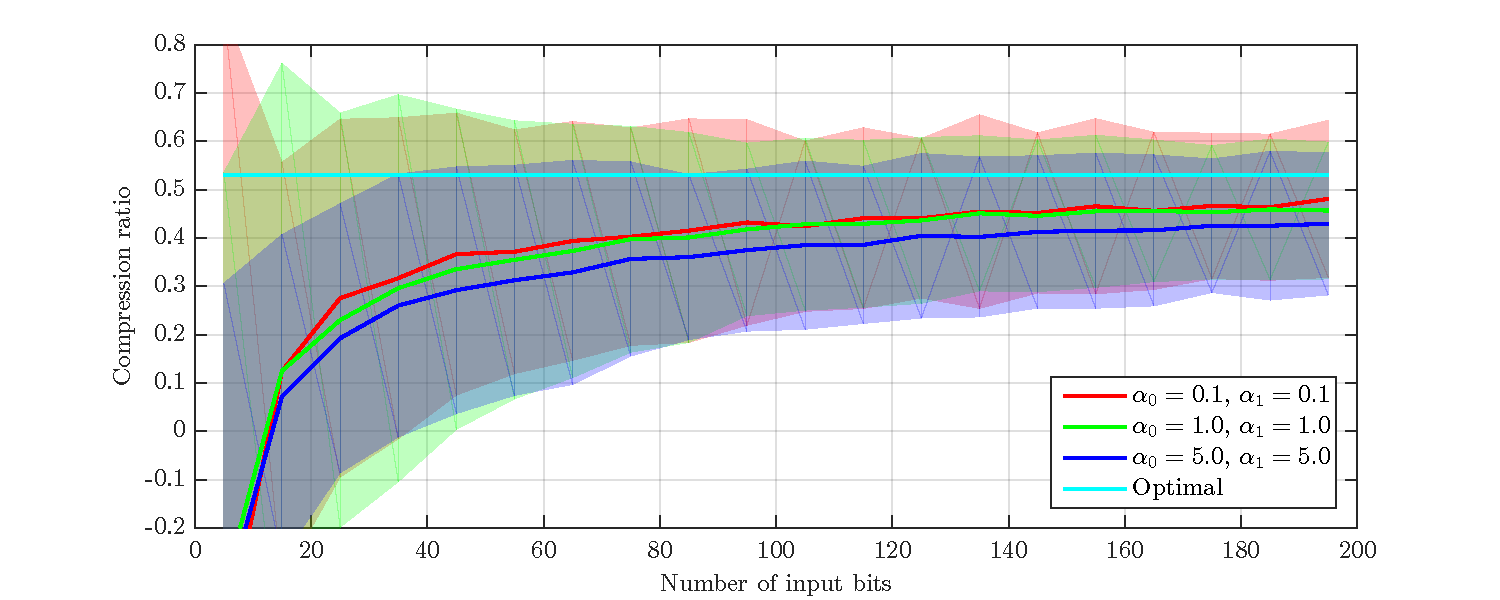
\includegraphics[width=.95\linewidth]{\outputPath old/comparison_priors}
    \caption{Comparison of the adaptive compression scheme for different $\alpha_0$ and $\alpha_1$ when the input is fed bit by bit. The lines and associated areas show respectively the means and 95\% confidence regions determined over 50 runs.}
    \label{fig:comparison_priors}
\end{figure}

\endgroup
\printbibliography

\end{document}
